\documentclass[11pt,a4paper]{article}
\usepackage[T1]{fontenc}\usepackage[utf8]{inputenc}\usepackage{lmodern,geometry,hyperref,tikz}\geometry{margin=22mm}\setlength{\parindent}{0pt}\setlength{\parskip}{5pt}\setlength{\emergencystretch}{3em}
\begin{document}\section*{SMC\_02: követelmény--komponens--teszt bizonyítéklánc}
Létrehozva: 2026-10-15 12:22 +02:00. ETA: 60--90 perc; meglévő két sablon bővítése, korlátozott profil validált projekciója, három nézet és ellenpéldák, kézirat/PDF.
\paragraph{Cél és határ.} A robotemitter-javítások megőrzése. A második domén teljes azonosító-, attribútum- és relációhalmazát külön kézi referenciához és IR-lekérdezéshez hasonlítani. Allokáció, megvalósítás, tesztkapcsolat és rögzített teszteredmény külön fogalom. A teszteredmények szintetikus tanúadatok, nem hardveres igazolások. A SysML ellenőrzés deklarált szövegrészhalmazra vonatkozik, teljes natív SysML validátor nélkül nem állítunk eszközkonformitást.
\paragraph{Tulajdonosok.} Core: fordítás, kanonikus identitás, checked leaf updates és snapshot publikálás. Query: pontos vocabulary-ID alapú, olvasó trace projekció és szerepellenőrzés. Formats: validált facade, meglévő template-registry, CSV serializer/template és vékony példa. A profil egy scope-ba tartozó, egyedi ASCII nevű entitásokkal és kétpólusú bináris trace-élekkel dolgozik; a más alakú bemenet explicit hiba, nem csonkolás. A két azonos végpontú, külön nevű él külön marad.
\paragraph{Változtatások.} Query traceability modul és export; Formats traceability facade, export, új CSV transform regisztráció; meglévő requirements SysML/DOT query és template; meta\_sysml\_trace vocabulary test\_case/verifies elemei; traceability\_verification fixture; Formats traceability teszt és példa; meglévő Query trace regressziók szükséges aktualizálása; tools/traceability oracle/checker; README célzott kiegészítés. A pontos fájllista a before-files.json-ban. Kézirat: codegen/evaluation/conclusion/supplement és a hozzájuk kapcsolódó abstract, bizonyítékmanifest. Új terv és PDF/JSON/ábra a dátumos reports alatt.
\paragraph{Szerződés.} A publikus facade csak validált profilt exportál, a generikus templater önmagában nem ilyen domainvalidátor. Nincs új parser, IR, hash vagy saját snapshot implementáció. Nincs új csomagfüggőség, CORE.YAML=[]; nincs RL, fizikai időléptetés vagy sebességmérés. A régi trace-witness eredmények történeti adatok, a hibás allokáció=megvalósítás olvasat pontosítandó.
\paragraph{Ellenőrzési mátrix.} Teljes modell; checked eredménymódosítás; strukturális követelmény/komponens/teszt hozzáadás; visszatartott régi snapshot; hibás szerep, semleges/extra résztvevő, két arc, azonos név más scope-ban, veszélyes szöveg, hibás teszteredmény elutasítása. A három nézet külön visszaolvasója minden teljes relációt összevet Q(H)-val és kézi JSON-nal. Hiányzó nézet, törölt/duplikált/felcserélt él, megváltozott attribútum, mindhárom nézet közös hibája és elavult nézet nem lehet PASS. A lefedetlen/failed/unknown követelmények pozitív diagnosztikai kontrollok. Régi emitter/MJCF regressziók megmaradnak.
\paragraph{Erőforrás és skálahatár.} Legfeljebb 4 Cargo-job, kicsi determinisztikus helyességi példák; nincs benchmark. A projekció lineáris leltárt és indexeket használ, nem készít n-áris Descartes-szorzatot. Exportált fájl csak új célkönyvtárba; a forrás vagy kimenet nem váltható át csendes fallbackre. A nagy ipari modellek és általános SysML támogatás külön vizsgálatot igényelnek.
\paragraph{Visszaállítás és lezárás.} Csak a mentett saját diff; korábbi robotjavítás, párhuzamos Dynamics és kéziratmódosítás megőrzendő. Nincs commit/push/merge/branchváltás. Szűk tesztek, Clippy/formázás, forráshash-ek, teljes parancsok, PDF és archivált byte-egyezés. A jelen feladat nem a baseline összehasonlítás és nem clean-clone release.
\begin{center}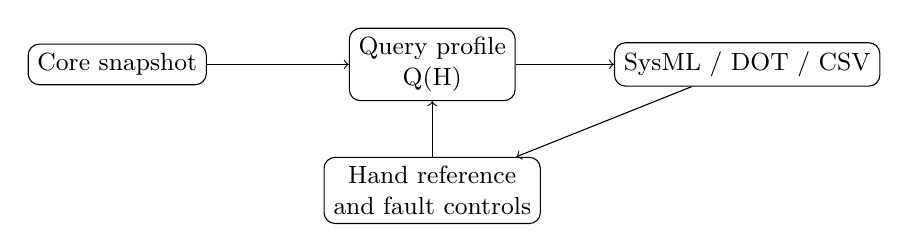
\begin{tikzpicture}[every node/.style={draw,rounded corners,align=center,font=\small}]\node (h) at (0,0) {Core snapshot};\node (q) at (4,0) {Query profile\\Q(H)};\node (v) at (8,0) {SysML / DOT / CSV};\node (o) at (4,-1.6) {Hand reference\\and fault controls};\draw[->] (h)--(q);\draw[->] (q)--(v);\draw[->] (o)--(q);\draw[->] (v)--(o);\end{tikzpicture}\end{center}\end{document}